\chapter{Interlude: Dewarp}

\begin{wrapfigure}{O}{\figwidth}
	\begin{center}
		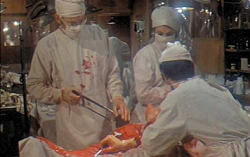
\includegraphics[width=\figwidth]{pics/13/1.png}
	\end{center}
\end{wrapfigure}
Doc was in his element. 
Well, actually he was in the Occurrence Border's medbay and up to his elbows in the guts of a very unhappy armsman, but same difference. 
All around him people were shouting, screaming, and generally running around in a blind panic, but he was the calm little center of the universe. 
Doc hummed to himself as he dug around, and then let out a shout of a triumph as he finally found the foreign object. 
It looked to be a large metal rivet, and still tingled with traces of the burst of warp-energy which had propelled it. 
He neatly tossed it into the prayer-seal covered bin marked "Tainted," and began closing everything back up.

As Doc moved on to his next patient he allowed himself a moment of pride. 
Despite his complete lack of official medical education, he liked to think that he was a master when it came to Meatball Surgery. 
He shot a glance across the room towards where the chief medical officer, Sister Valerie of the Ordos Hospitaller, was dealing with the non-trivial patients. 
Their eyes met for a second and Doc smiled as he looked back down to inspect his new patient's severed arm. 
Then a painfully-shrill screech rose from the waste bins, the lights and gravity both cut out, and a medical cogitator in the back of the medbay began frantically beeping.

Doc automatically turned his shoulder tac-light on, snatched the now-floating severed arm out of the air and instructed his patient to "keep a hand" on it, and drew his sidearm. 
The minor daemon that clawed out of the medical waste bin, already weakened by the prayer seals, was dispatched with single volley from Doc's las-pistol. 
That minor annoyance dealt with, he disengaged his mag-boots and launched himself towards the back of the medbay. 


\begin{wrapfigure}{O}{\figwidth}
	\begin{center}
		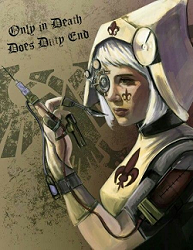
\includegraphics[width=\figwidth]{pics/13/2.png}
	\end{center}
\end{wrapfigure}
Sergeant Gravis of the Emperor's Scythes Space Marines, or more specifically the upper-half of Sergeant Gravis, twitched as the Tyranid bio-weapon in his veins made another spirited attempt to kill him. 
The medical cogitator hooked to him requested several types of antidote, which Doc quickly administered.

"We're down to our last vial of Hydroxocobalamin, and he's having nightmares again" reported Doc. 


Sister Valerie didn't look up from her patient as she responded. 
"The warp's a bad place to be comatose, especially this far from the light of the Emperor, and the way that unholy xenos abomination is tearing apart the ship doesn't help. 
He's not the only one who'll die if we don't return to normal space soon either."

"I swear honey-" 

"Ma'am" 

"-Ma'am, Sarge said we'll be reaching the waystation today, then we can request all the aid and supplies we need. 
Just a little longer and it'll all be over."

As Doc finished stabilizing the Space Marine and made his way back to the table he'd been working at, the medbay's lights reactivated. 
A second later, the was a clattering crash as the various small items that'd been floating through the air dropped back to the floor, and a meaty thump as Doc's neglected patient was slapped by his own severed arm.

Sister Valerie watched for a second as Doc hastily apologized to the maimed crewman and scrambled under the table for the dropped limb. 
In a voice too quiet for even her nurses to hear, she muttered, "Emperor… why'd he have to be an optimist?"

\greentext{>The All Guardsmen Party Interlude: Dewarp}


\begin{wrapfigure}{O}{\figwidth}
	\begin{center}
		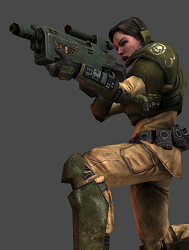
\includegraphics[width=\figwidth]{pics/13/3.png}
	\end{center}
\end{wrapfigure}
Amelia Delorisista Amanita Trigestrata Zeldana Malifee von Humpeding was on the hunt. 
The creature that had been haunting the aft tainted areas and attacking unwary crewmen and servitors had eluded them for days, but now she had it.

Aimy readied her pulse-rifle as her bait slowly advanced into the disused cargobay and her spotter scanned the area. 
It was a perfect example of the classic monster-hunting technique, or it would've been if the bait stopped whining.

"I don' see  why I aways gos'ta be da bait" whinged Nubby. 
"I fink it's discra-, err dissema-, err distra-, err unfair. 
I fink it's unfair."

Aimy didn't respond, but her goggle-clad spotter suggested that it wasn't discrimination: 
Nubby just needed to stop picking rock every time.

Nubby's complaints rose in volume as he began arguing with Fumbles over the rules of a game older than the Imperium of Man. 
"It's not right 'ow paper beats rock. 
Wrappin around it... 
where's da sense in dat? 
Still a rock ainit? 
Jus' all wif paper n stuff."

Things got even louder when Twitch commed in and began explaining the the game was actually a metaphor for the relationship between the Ecclesiarchy, Administratum, and Mechanicus. 
Eventually, the argument was cut short as Aimy lost her patience. 
A few inventive, and highly-personal, death-threats later, the team fell back into silence and Nubby "got on with it".

"Oh woe is me, I am poor an' fenceless 'uman wot 'as lost 'is way in dis 'ere big an spooky cargobay. 
I sure 'ope dere's not some sor' of ten-ack-ulled warp-mon-strosi'y lurkin down 'ere an' waitin ta eat me."

Fumbles peered into a dark corner of the bay as Nubby monologued. 
He could sense a malevolent presence that just barely qualified as a mind moving closer, and pointed it out to Aimy. 
The Markswoman sighted her rifle on the corner, and waited for the creature to make its move. 
"Still not sure what it is Fumbles?" The psyker sheepishly shook his head.

\begin{wrapfigure}{O}{\figwidth}
	\begin{center}
		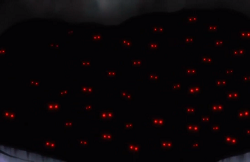
\includegraphics[width=\figwidth]{pics/13/4.png}
	\end{center}
\end{wrapfigure}
"Well, at least it can't be that smart if it's falling for this" Aimy gestured towards the soliloquizing bait. 
"Though I gotta say his performance is better than usual. 
The wig and dress are a nice touch."

Fumbles nodded in agreement, "He says they help him get into character."

"It really says something that I don't find this conversation even remotely weird..." Fumbles just shrugged, and there as a brief silence as Aimy shifted mental gears. 
"You know, my life was really quite boring before I joined the Inquisition. 
Mother never let me up on the lines when there was something really interesting to shoot."

Aimy felt a pang of longing that definitely didn't originate from her, "Sounds nice. 
Wish I'd had parents." muttered the psyker.

Aimy glanced up from her scope, "You can be really fucking depressing you know."

"Sorry."

"Whatever. 
You got any idea why this thing isn't coming out? 
Does it know we're here?"

Fumbles pondered the question before answering, "No, I think it's waiting."

"Waiting for wh-"

Aimy was interrupted by a sudden pain in her head, a panicked scream from Fumbles, and the sudden absence of both light and gravity. 
In the completely dark cargobay, Nubby's well-honed survival instincts kicked into overdrive as first one, then two, then a dozen chittering screeches rose around him. 
Before Aimy had even reoriented herself, the be-dressed little trooper, screaming shrilly and propelled by the recoil of his Pulse Carbine, shot past her and slammed into Fumbles.

Nubby, dragging the semi-conscious Fumbles with him, started bouncing his way down the corridor with all the speed provided by his his augmetic legs, leaving Aimy struggling to catch up. 
As she flew, Aimy shined her rifle's tac-light back towards the cargobay and saw the forms crawling along the floor, walls, and ceiling. 
She started firing her rifle, just for the little bit of extra speed, and screamed "PLAN B!" into her combead.

At the far end of the corridor, Twitch smiled.
\begin{wrapfigure}{O}{\figwidth}
	\begin{center}
		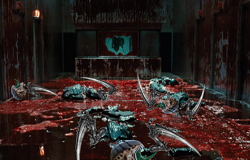
\includegraphics[width=\figwidth]{pics/13/5.png}
	\end{center}
\end{wrapfigure}
When the ship's lights reactivated a few minutes later, they revealed a shrapnel-pocked corridor filled with a disgusting cloud of limbs and juices. 
Twitch re-opened the door the four of them had sheltered behind and surveyed the carnage. 
As Aimy drifted over to join him at the doorway, Twitch felt something shift and flung himself behind the markswoman. 
A second later, the gory mess hanging in the corridor dropped out of the air with a horrible splash.

Aimy sputtered and swore, Nubby laughed, and Twitch peeked around his human shield. 
Sure that the coast was clear, the demolitions trooper crept forward. 
He poked at the horrible slurry, carefully pulled a large chunk out of the mess, and then started giggling. 
Nubby took a break from checking Fumbles' health using the tried and true Guard technique of gently kicking him in the ribs while muttering "yous okay?" to ask Twitch what was so funny.

Twitch turned a manic smile on Nubby. 
"These weren't daemons!"

"I swear, if you try to tell us those were Orks, I will cram your delusional little head up your ass," growled Aimy. 


Twitch bristled at this. 
"I don't ALWAYS say it's Orks."

"Yeah you do," inserted Nubby.

"Well, I'm not saying it's Orks this time."

Aimy picked an especially large chunk off her armor. 
"Good, because if you've just covered me with Ork-guts again, I'll have to kill you."

"Deaf frets aside, I fought Fumbles 'stablished dat dese were daemons. 
Ain' dat right buddy?" Nubby's metal foot prodded Fumbles again, eliciting a pained groan. 
"E says yes."

Twitch responded by yanking Nubby away from the suffering psyker, and shoving the limb he'd acquired into the trooper's face. 
Nubby went crosseyed as he stared at the razor-sharp limb, then swore. 
Aimy came over and swore too.

After a brief silence, Twitch spoke, "We gotta call Sarge."

"E's not gonna like dis…" muttered Nubby, "NOT IT!" 

"NOT IT!" echoed Twitch.

*BLARF* added Fumbles.

Aimy glared at them, and keyed Sarge's channel.

\begin{wrapfigure}{O}{\figwidth}
	\begin{center}
		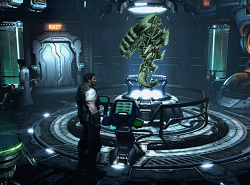
\includegraphics[width=\figwidth]{pics/13/6.png}
	\end{center}
\end{wrapfigure}

Deep inside the spacefaring pile of scrap known as the Occurrence Border, there is a circular room filled with arcane machinery. 
In the middle of this room is a bubble of blue light which contains a large xenos that resembles a cross between a snake and a nightmarish fetus. 
The xenos is a type of potent Tyranid Psyker known as a Zoanthrope, which was captured in a daring Space Marine assisted raid, and is now being transported to an Inquisitorial laboratory for study.

The imprisoned Zoanthrope is being held completely still by a stasis field, but its sheer psychic presence distorts the world around it, and acts as a beacon to the denizens of the warp. 
The kludged-together Psyker Containment Area is straining to shroud the xenos' presence from the daemons surrounding the ship, and limit the power of the creature's mind. 
Every single sub-system is on the ragged edge of failing, some are sparking, others are smoking, and the Stasis Unit itself is emitting an ominous hum that steadily rises in pitch.

Two men, one in a filthy Guard uniform and the other sporting the robe and augmetics of the Adeptus Mechanicus, and a Tau of the Earth Caste variety are running around in a constant effort to repair the Containment Area's failing systems. 
A third man, whose uniform and bearing scream NCO, is standing directly in front of the Zoanthrope, and holding what appears to be a piece of hull-plating like an oversized shield.

The shieldbearer is Interrogator Greg Sargent, and he is not having a good day.

\begin{wrapfigure}{O}{\figwidth}
	\begin{center}
		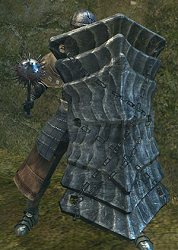
\includegraphics[width=\figwidth]{pics/13/7.png}
	\end{center}
\end{wrapfigure}
Sarge tightened his grip on the massive shield as the Stasis Unit's humming reached a painfully high pitch, then went out of the range of human hearing. 
After a few tense seconds there was deafening *CLANG*, and the blue field around the Zoanthrope disappeared. 
It was immediately replaced by a corona of green electricity, which gathered in front of the xenos as it turned to face the frantically working Fio. 
With a scream of effort, Sarge hefted the shield and sprinted across the room, barely managing to intercept the lightning bolt in time.

Without a second of hesitation, the Zoanthrope began gathering another bolt of electricity and twisted around to face the opposite side of the room. 
Sarge lifted his smoking shield for another sprint, but let it drop back down to the floor as the Stasis Field snapped back into existence. 
Behind him, the squat Tau scientist complained that Sarge was standing in his light.

At the sound of Sarge grumbling about the "Ungrateful little xenos bastard," Tink looked up from the mess of wires he was digging through. 


"Hmm? 
Oh, nice catch boss, we'd all be dead without you. 
Truly, you're a master of standing in front of things. 
Now, since you're just standing there, can you grab me another handful of triplex connectors? 
Next flicker should be in three minutes, you've got time."

Sarge glared at the techie, but set down his shield and headed off to get the requested parts. 
On the far side of the room, Chief Enginseer Jim leaned out from behind a glowing blue pylon, and angrily waved a mechadendrite.

"DAMNIT TINK! 
No more triplex connectors, they anger the machine-spirits, stick to duplex."

Tink scoffed, "Machine spirits my ass, they work FINE! 
Come on Fio, back me up on this."

The Tau responded without looking up from his work "There's no scientific reason triplex connectors shouldn't work. 
They're completely compatible with duplex systems, and are, in fact, rated to a much higher capacity."

"See!"

\begin{wrapfigure}{O}{\figwidth}
	\begin{center}
		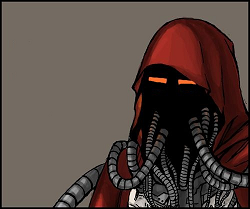
\includegraphics[width=\figwidth]{pics/13/8.png}
	\end{center}
\end{wrapfigure}
Jim returned to his work with a few mutters about his poor, abused machines, and Sarge delivered the controversial parts. 
As Sarge hefted his massive shield and got into position, the Stasis Unit began making its ominous humming again and Tink rushed to finish his repairs. 
With a shout of triumph, he reconnected the final component, slammed the panel shut, and ran over to one of the control panels lining the room.

The mental pressure everyone in the room had been feeling quickly decreased. 
Sarge let out a sigh of relief, Tink cheered again, and Fio asked if anyone else could smell smoke. 
A second later the panel Tink had just shut was flung across the room by a small explosion, and the mental pressure returned with painful intensity. 
From behind his pylon, Jim shouted "I TOLD YOU THEY DON'T LIKE TRIPLEX!" 

While the three techies ran around in a panic, Sarge stood still and watched the Stasis Unit. 
He looked down at his shield, up at the green aura that was gathering around the Zoanthrope despite the temporarily-functional Stasis Field, back down at the shield, and reached a decision. 
Silently counting to himself, Sarge raised the massive slab of metal over his head.

Sarge didn't wait for the Zoanthrope to make the first move: 
as the Stasis Field cut out, he flung the heavy shield with all his beefy-noncom strength and dove for cover. 
There was a *CLANG* followed by a *ZAP*, a *THWAP*, and a massive, crackling *BOOM*.

For a split second the room was lit by a blinding green light, and then everything went dark. 
Sarge hung in the air at the apex of his jump, and blinked in the pitch darkness. 
He wondered if he'd finally gotten himself killed, and whether the afterlife truly involved fighting by the Emperor's side, or if Twitch was right about the poker room. 
Then he crashed into the ceiling and the ringing in his ears faded into Jim screaming at Tink about how he'd caused a ship-wide power outage with his damned triplex connectors.

\begin{wrapfigure}{O}{\figwidth}
	\begin{center}
		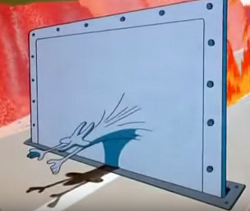
\includegraphics[width=\figwidth]{pics/13/9.png}
	\end{center}
\end{wrapfigure}
Since he was apparently still alive, Sarge decided it was a good idea to stay that way and turned on his tac-light. 
He tried to twist around to face the Zoanthrope, but this turned out to be rather difficult, since the Stasis Unit was now empty. 
After a brief period of panic, Sarge realized that the lack of green lighting bolts meant that the xenos wasn't currently up for a fight, and began carefully scanning the room. 


Remembering the meaty thunk he'd heard after throwing the shield, Sarge aimed his light at the far side of the room. 
It revealed a horrible form made of chitin and metal hanging in the entrance of the debris-clogged cell. 
A closer look revealed it to be the Zoanthrope, except with a partially-melted shield wrapped around its head. 
Sarge floated over and scientifically poked it with his gun, took its feeble twitching as a good sign, and began hefting the xenos out of the cell and back towards the Stasis Unit.

While Sarge wrangled the Zoanthrope back into place, Tink, Jim, and Fio climbed around the incredibly deep hole that occupied Sarge's former position. 
From the very bottom, Fio could be heard complaining that whoever had installed the wiring in his section had not been a sept-certified electrician. 
Jim, who was patching cables slightly higher up, suggested that the person had probably been either drunk, or insane, or both. 
At the top of the hole, Tink reconnected a group of wires with a few duplex connectors, and nearly wet himself when the tangled mass started sparking and the room's com-terminal chimed.

At the sight of the familiar contact code on the screen, Tink launched himself out of the hole and flew over to the terminal, ran a hand through his filthy hair, straightened his goggles, and oh-so-casually answered the incoming call. 


"Heyyyyyy Hannah, what's up baby?"

Sarge heard the enraged screeching from across the room, but couldn't make out any worlds aside from "stupid" and "insane".

\begin{wrapfigure}{O}{\figwidth}
	\begin{center}
		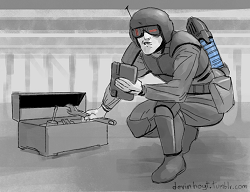
\includegraphics[width=\figwidth]{pics/13/10.png}
	\end{center}
\end{wrapfigure}
Tink continued undeterred, "Why would you assume I had anything to do with this? 
Is it because you're always thinking about me?" 

This time the screeching was accompanied by a short arc of electricity. 
Cursing and clutching his burned ear, Tink floated away from the terminal, and then crashed to the ground next to the hole as gravity and light returned to the cells. 
After a feeble attempt to climb to his feet, the techie gave up, leaned over the side of the hole, and groaned "Hey Jim, your sexier counterpart is being all bitchy. 
You can talk to her."

While Jim climbed out of the hole and began giving a damage report to Hannah, Sarge pushed the Zoanthrope back into the network of grav-plates above the Stasis Unit. 
Once he was certain the now-metal-faced Xenos wasn't going anywhere, Sarge dragged Tink up off the floor and over to the non-functional Stasis Unit. 
A few kicks and death threats convinced the techie that getting the Stasis Field back up was more important than eavesdropping on Jim's conversation, and the two guardsmen got to work. 


Right as the last fixes were being made, Sarge's combead came to life with the sound of Doc's slightly-panicked voice. 
"Hey Sarge, the Captain's been trying to reach you over the ship's comms, he says we're there."

With a rare smile, Sarge relayed the good news to the combead-less Tink, who practically collapsed with relief and leaned towards Sarge's headset "Oh thank the Emperor, Doc tell him we'll be ready in five minutes." 

On the far side of the combead, Doc's voice grew a little panicked, "Umm, I don't think you've got five minutes, I think he meant we're THERE there, as in we're dewarping RIGHT NOW." Sarge winced as Tink ripped the combead off his head and began screaming into it.

"WHAT HAPPENED TO OUR WARNING DOC? 
I WAS PROMISED A FIFTEEN MINUTE WARNING!"

\begin{wrapfigure}{O}{\figwidth}
	\begin{center}
		
\includegraphics[width=\figwidth]{pics/13/11.png}
	\end{center}
\end{wrapfigure}
"How should I know?" responded Doc, "I'm just passing the word along. 
All I know is that the Captain said your room's comm is busy and asked me try and reach you."

"That's totally not my fault." Tink shot a glare towards the room's com terminal where Jim was chattering about catastrophic system damage with Hannah, and then returned his attention to the combead. 
"And why didn't he just call us like you did?"

Doc's tone shifted from panicked to annoyed. 
"Maybe because you helped Twitch encrypt all of our combeads day before yesterday."

"That was just to keep the cogboys from spying on us, and he said he'd share the code with everyone who needed it!"

There was a brief pause as Doc digested this, then the medic exploded. 
"YOU thought HE'D share the code? 
This is TWITCH we're talking about you idiot, OF COURSE HE DIDN'T SHARE IT WITH ANYONE!"

Tink began putting together a suitably scathing response, but was interrupted as Sarge wrenched the combead back and spun him around to face the psi-suppressors. 
"Talking time over, fixing time now! 
MOVE IT TROOPER!" 

Once he was sure Tink was back on task, Sarge turned his attention to Jim. 
Using his refined oratory and leadership skills, he convinced the techpriest that repairing the cells' various delicate systems before the stress of de-warping blew them into shrapnel took priority over helping Hannah with the ship's power problems. 
Which is to say: 
Sarge reached over Jim's shoulder and terminated his call, then picked the hapless Enginseer up by his crimson robes and flung him towards Tink with a shout of "FIX STUFF BEFORE IT EXPLODES!"

As two techies scrambled, and Fio asked what was going on and if anyone could help him out of the hole, Sarge entered the bridge's contact code into the comm terminal. 
Unfortunately, his plan to yell at the Captain for attempting to get them all killed ran into problems when the ex-navy officer answered the call with a bellow of "WHY IS MY NAVIGATOR UNCONSCIOUS, SARGE?"

\begin{wrapfigure}{O}{\figwidth}
	\begin{center}
		
\includegraphics[width=\figwidth]{pics/13/12.png}
	\end{center}
\end{wrapfigure}
Back in the aft of the ship, Aimy's combead nearly deafened her as it finally connected to Sarge's. 
After a few attempts to make herself heard over her boss' shouting match, she removed the earpiece and turned to her companions. 
"I think he's busy, apparently we're all about to die."

Nubby, seated on Fumbles' curled up form, paused in rummaging through a medkit that appeared to be filled with nothing but lho sticks and suspiciously-unlabeled bags of pills. 
"Huh… neat. 
Anyone wanna smoke?" Behind him Twitch reacted a little more strongly, leaping to his feet with his rifle in one hand and grasping for some something inside his jacket with the other. 


"I knew it! 
Have we been boarded? 
Who's coordinating the defence? 
Should I blow the ship's plasma reactor before-" His tirade was cut off as Nubby yanked the detonator out of his hand and began dancing backwards down the hall with it.

Aimy listened a little longer, then called after the pair, "No boarders, but he's arguing with the Captain about whether to stay in the warp and risk the Navigator getting possessed, or dewarp and potentially blow up the Cells."

Nubby paused for a second, "Speakin as someone oo's nowhere near da Cells, I vote for dat one." Twitch seized on Nubby's distraction and made another grab for the detonator, but Nubby managed to spin away and crammed it down between the two wads of dirty socks holding up the front of his dress. 
This did not deter Twitch even slightly. 
Aimy gagged a little and Fumbles laughed weakly as Twitch tackled Nubby to the ground and began rooting around for the detonator.

As Twitch finally found his prize and withdrew it (along with a handful of crusty socks), a deep vibration came up through the floor and the vox system began blaring the completely-incomprehensible automated de-warping warning. 
Aimy raised her combead back to her ear, Twitch and Nubby both cheered, Fumbles began whimpering again, and back in the gore-filled hallway something moved.

\begin{wrapfigure}{O}{\figwidth}
	\begin{center}
		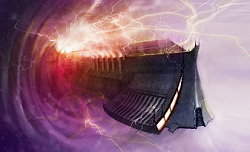
\includegraphics[width=\figwidth]{pics/13/13.png}
	\end{center}
\end{wrapfigure}
Tink and Jim worked feverishly. 
In the background the automated de-warp warning instructed all hands to hold still and pray to the Emperor in thirty-six different variations of Gothic (not to mention Jantine Battle-Cant and what the resident xenologist insisted was Hrud), until Sarge used his carbine to deactivate the nearest speaker. 
The noise of the de-warp warning was replaced by the pops of overloading psi-suppressors, Fio's demands to be told what was happening, and the sound of Sarge yelling at the Captain to slow down. 
Inside the inactive Stasis Unit, unnoticed by everyone, the Zoanthrope began twitching.

Doc threw himself across the medbay as Sergeant Gravis went into double-cardiac arrest. 
While he struggled to fight the increasingly active tyranid bio-weapon, the deep vibration of the ship's Warp Drive grew stronger and stronger.

Aimy, Twitch, and Nubby all flinched as a sensation similar to fiberglass being rubbed on exposed nerves shot through their heads, and automatically turned to face Fumbles. 
Aimy got as far as "THE FUCK IS WRONG WITH YOU NOW-" before she noticed the way the gore in the corridor had begun to bubble and froth. 
With remarkable coordination, the three troopers seized Fumbles and started retreating down the now-wildly-shaking corridor. 
Then, right as they reached the next door and turned back to see what they were running from, the vibrations stopped with a colossal, tooth-rattling *CLANG*.

\begin{wrapfigure}{O}{\figwidth}
	\begin{center}
		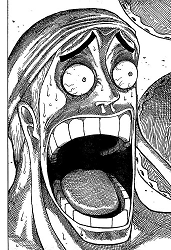
\includegraphics[width=\figwidth]{pics/13/14.png}
	\end{center}
\end{wrapfigure}
Twitch swore, Nubby screamed, Fumbles started twitching madly, and Aimy looked around in confusion. 
She got as far as "What the f-" before all the gore, including the portion soaking her armor, suddenly ran together and reformed into familiar insectoid shapes in a sort of reverse-explosion. 
All three troopers immediately opened fire.

As the *CLANG* reverberated through the medbay, Doc went pale. 
Sister Valerie met his gaze from across the room and began to ask "What the f-", but her question was interrupted as the ragged edge of Gravis' torso inexplicably burst into green and black flames. 
Sister Valerie abandoned her current patient and sprinted towards Gravis as Doc screamed "THIS IS NOT HOW POISON IS SUPPOSED WORK!", and grabbed a fire extinguisher off the wall.

As the echoes of the *CLANG* died away, Tink leaned out of the cover he had jumped into when the  psi-suppressor he'd been working on exploded. 
"What. 
The FUCK. 
Was THAT?" asked the shaken techie. 
Jim didn't respond, being rather busy rocking back and forth and whimpering to himself, and Fio rather crossly asked how someone stuck in a hole was supposed to know anything about what was going on.

Sarge raised his Carbine with a mutter of "Oh not this shit again," and began scanning the room. 
Behind him the comm terminal chimed as another person joined the call, and the husky old voice of Ol' Bill temporarily overrode the Captain's demands for information. 
"Hey guys, know you're busy screamin at each other, but we've got something big and psychic holdin us in the warp. 
Either of you seen any major daemons running around? 
Or is this just your damned bug again Sarge?"

Sarge focused on the twitching Zoanthrope and took a step forward, "I think it might be the..." The xenos psyker snapped its metal-covered face towards him, surrounded itself with a halo of green and black electricity, and a tide of insects began pouring out of every crack in the room. 
"DEFINITELY THE BUG!" shouted Sarge.

\begin{wrapfigure}{O}{\figwidth}
	\begin{center}
		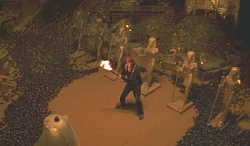
\includegraphics[width=\figwidth]{pics/13/15.png}
	\end{center}
\end{wrapfigure}
Sarge dropped his carbine onto its sling and sprinted for the Stasis Unit, crushing insects under his boots as he ran. 
For a second the room around him seemed to stretch and warp, but it stopped as Jim snapped out of his funk and plunged his mechadendrites into one of the psi-suppressors. 
Several small bolts of green and black electricity grounded on Sarge as he finally neared the Stasis Unit, but he ignored them and triumphantly flipped the big switch to ON. 
Nothing happened. 
Sarge frantically flipped the switch up and down, and screamed "I THOUGHT WE FIXED THIS, TINK!"

Tink slammed into the unit next to him, slapped his hand away then set the switch to on, and responded with forced calm "Had to replace the capacitors to fix the flicker, they need to char-AGHHHH." Tink's calm tone evaporated as the began slapping at the insects that had just crawled up his pants leg. 
Sarge sprang to help, then noticed the way the insects were flowing towards the open maintenance panel on the Stasis Unit. 
He immediately began employing his big, stompy boots in an effort to stem the tide, screaming at Tink as he did so. 
"WHY DIDN'T WE TURN IT BACK ON AFTER WE FIXED IT?"

"BECAUSE WE'RE IDIOTS SARGE!" responded the techie as his frantic dancing finally dislodged the last bug and he joined Sarge in stomping the on-rushing swarm. 
Even with two sets of boots, it was obviously a losing battle, but being Guardsmen, neither of them commented on this. 
They continued in their desperate attempt to Hold The Line, as the tide surrounded them and began climbing both their legs and the Stasis Unit. 


Across the room, Jim noticed their predicament and, in a fit of genius, scrambled over to Fio's hole. 
He very calmly asked the Tau to redirect extra power from the damaged suppressors to the Stasis Unit. 
There was a flash of blue light behind Sarge and Tink, and both of them collapsed as the universe twisted and what felt like a million barbed legs ripped across their minds.
\begin{wrapfigure}{O}{\figwidth}
	\begin{center}
		
\includegraphics[width=\figwidth]{pics/13/16.png}
	\end{center}
\end{wrapfigure}
For the second time that day Sarge wondered if he'd been killed, but as the empty ringing in his head was replaced by what felt like the universe's worst hangover, he decided that he was probably still alive. 
He just wished he wasn't. 


Moving with the extreme care of someone with a near-terminal headache, Sarge sat up and looked around the Cells. 
Surprisingly, things looked more-or-less stable. 
The bugs were gone, though his legs felt like they'd been worked over with a wire brush, and a certain feeling in his gut told him the Occurrence Border had finally exited the warp. 
It seemed that without the strain of traveling through that hellish realm, the few still-functional psi-suppressors were holding up fine. 
Well, as far as he could tell they were fine... 
at least none of them were on fire, and whatever Tink had done to the Stasis Unit had fixed that damned flicker. 
Sarge eyed the stationary Zoanthrope and its creepy new metal-covered face, then flipped it off and turned his attention to his team.

Tink was curled up nearby, clutching at his head and alternating between crying and swearing. 
Jim was already back on his feet and doing techpriest things, and Fio had finally hauled himself out of the hole in the floor. 
The annoying little xenos looked rather confused about what had happened, but had just enough self preservation instinct to go help Jim instead of bothering Sarge or Tink with questions. 
Sarge decided that the situation was stable enough for the time being, and carefully lowered himself back down to the floor, only to be jerked back upright as a something drove a red-hot poker into his head via his ear. 
He frantically reduced the volume on his combead until the voice coming through it changed from a horrible daemonic screech made of pure agony, to Doc's rather worried tone.

\begin{wrapfigure}{O}{\figwidth}
	\begin{center}
		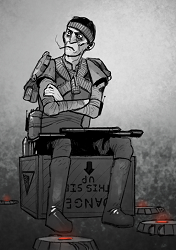
\includegraphics[width=\figwidth]{pics/13/17.png}
	\end{center}
\end{wrapfigure}
"You alive Sarge?"

"Sorta..."

Sarge flinched as Aimy's considerably louder voice joined the conversation. 
"What the hell happened down there?"

"Tink broke something." muttered Sarge with a halfhearted glare at the prone techie. 


Tink stopped moaning about his head, and dug through his gear pouches for his own combead, whining to himself as he searched. 
"S'not my fault, stupid machine spirits being little bitches. 
No bloody scientific reason…"

Sarge returned his attention to his combead and summoned up as much professionalism as he could manage. 
"Everyone still alive? 
Report."

"I'm fine, and Gravis is still alive, if a little crispy around the edges." replied Doc.

Aimy spoke next. 
"We're all okay, but the thing hunting people in the aft tainted area turned out to be a swarm of gaunts."

Sarge winced. 
"Oh, shit."

Aimy began to continue, but Twitch's voice, which sounded dangerously excited to Sarge's experienced ear, overrode her. 
"I was ready for that though, and we blew them into chunky salsa, except-" There was a brief scuffle in the background as Aimy explained to Twitch that interrupting was very rude. 


After a few seconds, Nubby awkwardly cleared his throat and continued the story. 
"Cept afta dat, all da bits n stuff stahted runnin togever an' dey got back up."

"Oh… shit…"

Aimy's voice returned. 
"But then we dewarped and they all sort of evaporated. 
Just POOF, gone. 
Blood, guts, and everything. 
So we figure-" Once again Twitch interrupted, "that the nids have formed an alliance with chaos! 
An unstoppable tide of Daemonids will sweep across the sector and- OW!"

Sarge sighed and rubbed his face as Tink and Nubby both snickered.

"We figure it was just some sort of warp-thingy. 
So, umm, I guess everything is fine. 
I mean Fumbles is unconscious, again, but otherwise everything is fine." finished Aimy, sounding rather annoyed over how her story had been spoiled.

\begin{wrapfigure}{O}{\figwidth}
	\begin{center}
		
\includegraphics[width=\figwidth]{pics/13/18.png}
	\end{center}
\end{wrapfigure}
Sarge ran through the whole disjointed report in his head. 
After a little pondering he held up his hand and began ticking off his fingers. 
"Okay, I guess we dewarped just in time to avoid that problem, so that's sorted. 
And it looks like the anti-psyker stuff is holding up fine now that we're out of the warp. 
And Gravis is still mostly alive right?"

"Right. 
Mostly." confirmed Doc.

Sarge looked down at his closed hand in surprise, ran through the list again in his head, then shrugged to himself. 
"So, uh, I guess we made it. 
I mean, here we are at waystation whatever. 
All that's left to do is requisition a few parts, drop Gravis off with the local medicae, get a new astropath, and call the Scythes. 
Then we spend a few leisurely weeks getting everything fixed up, and take a nice safe route back to wherever Oak's lab is." he paused for a second, not quite believing what he was saying, then continued "So yeah, we win, good job people…"

There were a few seconds of shocked disbelief, and then Sarge ripped off his combead as it exploded with cheers. 
When the volume finally returned to a safe level, he put it back on just in time to catch Doc say "You know, that trip went a lot easier than I expected."

"Oh shut up, you've been hiding in the medbay and sleeping in a nice warm bed every night," responded Tink in his most petulant voice. 
"I can't remember the last time I got to sleep for more than ten minutes."

Doc continued undeterred, "Okay, yeah, it was a bad week for some of us, I'll admit that, but it wasn't what I'd call 'hellish'. 
And 'hellish' is sort of the standard for our missions. 
I mean, when you look at it in comparison to some of our other assignments, this went amazingly well."

The was met with a thoughtful silence, which then slowly congealed as the squad followed the observation out to its logical conclusion. 
Eventually Twitch broke the uncomfortable silence. 
"Ohhhh we are sooo screwed. 
This one's going to be really, really bad."

\begin{wrapfigure}{O}{\figwidth}
	\begin{center}
		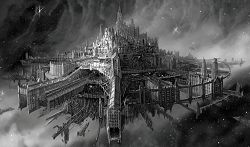
\includegraphics[width=\figwidth]{pics/13/19.png}
	\end{center}
\end{wrapfigure}
"What's going to be bad?" asked Aimy, revealing her inexperience.

"Everything."

"What?"

"It's like da third law of conservation of da fingy." translated Nubby, "Ya know 'Fer everyfing what appens, deres like, a completely dis-pra-portionate re-action'."

Sarge sighed, and translated the translation. 
"If your attack is going really well, it's an ambush."

"Wait, wait, are you guys seriously suggesting that nothing can possibly go right? 
That ANYTHING good that happens to us is just a setup for something especially horrible?"

"Yeah." "Yep!" "That's right." "Uh-huh." "It's been scientifically proven" responded the rest of the squad in unison.

"So what? 
There's some sort of all-powerful cosmic entity conspiring to make our lives as dangerous and miserable as possible for its own sick amusement?"

Nubby nodded, "Somfin like dat, or just, ya know, da uni-verse itself."

"I think it's the Orks" muttered Twitch.

Aimy ran the last few months through her mind. 
"That's... 
that's... 
surprisingly believable. 
Well not the Ork part, that's just retarded, but it makes sense." She paused, and applied this theory to the current situation. 
"Yeah... 
now that we've finally reached it, I can totally see this waystation being full of… of…" she trailed off.

"Chaos worshipping psychic mutants," suggested Twitch, "waiting to capture hapless visitors and overwrite their minds with copies of their cult leader's. 
Or Orks. 
Or Orks disguised as chaos worship-" Twitch was interrupted as Sarge, recognizing an unproductive line of thought, cleared his throat and rather wearily addressed his troops.

"Paranoia aside, we're just here for a nice, simple supply run. 
Everyone put together your shopping lists, and grab some rest while the Captain takes care of docking. 
And let's, PLEASE, just try to get through this without anyone blowing up the station, or being arrested, or assaulting someone, or committing tech-heresy, or... 
whatever it is you do to screw everything up Doc."